\chapter[SCP-066 埃里克的玩具]{
    SCP-066 Eric's Toy\\
    SCP-066 埃里克的玩具
}

\label{chap:SCP-066}

\begin{figure}[H]
    \centering
    
\includegraphics[width=0.5\linewidth]{images/SCP.066.jpg}
    \caption*{SCP-066, 在事故066-2发生前。}
\end{figure}

\bb{项目编号:}SCP-066

\bb{项目等级:}\dd{Safe} Euclid

\bb{特殊收容措施:}\dd{SCP-066应存放在Site 21的一个保险箱中。2级及更高级人员可在填写相关申请表后对SCP-066做实验。研究员可在实验日志066-Beta中记录结果。}

SCP-066应存放在Site 21的高价值物品储存设施中的一个碳化钨箱内。每个月必须人工检查一次该箱子有无内部损坏\footnote{SCP-066会一视同仁地毁坏任何装在其收容箱内的记录设备。};如果出现损坏,SCP-066必须被移至一个新箱子中。此任务由一条能够在三秒内完成任务的机械臂执行。

\bb{描述:}SCP-066是一团线编成的结构复杂的辫子组成的不定形物,重约一千克。SCP-066的线可以被单独抽出并操纵;这样做之后,对象将产生一个自然音阶上的音符(C-D-E-F-G-A-B)。

当产生一组六个或更多的音符时,SCP-066将产生性质和持续时间各不相同的良性效果。SCP-066在其产生的任何效果持续时不会对操纵作出响应。事件066-2之前,结果包括:

\begin{itemize}
\item SCP-066变成一只三色小猫,持续十七分钟。小猫显得非常友好和顽皮,看上去已被除爪和阉割。
\item 一首持续四分钟的歌,原音吉他配上歌手\slash 创作人{[}编辑]的歌声。歌词告诫听者在没有父母监督时不要使用尖锐锋利的物品。
\item 一个小纸杯蛋糕,巧克力味,覆有巧克力糖霜,顶上插有一根点燃的蜡烛。值得注意的是,在该效果之前产生的声音和《生日快乐》开头的调子一样。SCP-066在上述蛋糕被吃掉后恢复响应。
\end{itemize}

\bb{事件066-2:}2008年4月18日,D-066-4437用一把剪刀去剪下SCP-066的一部分以作测试。然而,当他开始剪的时候,SCP-066滚到离他一米的地方,发出一种未经识别的吱吱声。在得到进一步指示之前,D-066-4437尝试继续下刀,结果SCP-066再次滚走并发出这句话:“你是Eric吗?”D-066-4437否认后,SCP-066变成其当前状态(参见档案照片)并开始发出大声而不和谐的不连贯音符直至D-066-4437被带出房间。

\begin{figure}[H]
    \centering
    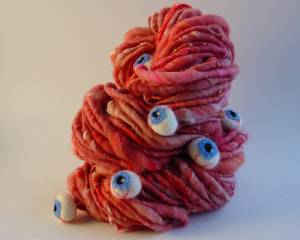
\includegraphics[width=0.5\linewidth]{images/SCP.066.2.jpg}
    \caption*{事件066-2之后的SCP-066。注:“眼睛”能够转动以跟踪运动和光源。 相片由\href{http://www.insubordiknit.com/}{Boggs特工}所拍摄。}
\end{figure}

事件066-2之后,SCP-066开始表现出和其原有特性高度不一致的行为。SCP-066现在表现出强大的移动能力,主要形式为能以极高的速度移动部分形体。当SCP-066不能或不想使用该能力移动时,它偶尔会尝试用线摩擦箱子内壁,逐渐使其磨损,以此来损坏收容。考虑到其构成材料,该过程异常有效。

除其移动能力外,SCP-066在任何人类在场时均会自行产生音符和效果,无论此人类是否与SCP-066互动。该过程似乎至少需要六秒钟。事件066-2后,SCP-066产生的效果包括:

\begin{itemize}
\item 在收容设施附近放出一只蜜蜂,飞走前蛰伤了D-4436。未捉住蜜蜂。不知道蜜蜂是如何存活的。
\item 贝多芬第二交响曲以超过140分贝的音量播放,造成三名人员永久失聪,另外八名人员听力永久损伤。
\item SCP-066的收容室突然完全失去光亮,持续五小时。室内人员称听到背后传来粗重的呼吸声,但找不到明显的来源。
\end{itemize}

当不产生异常效果时,SCP-066一直用低沉的男性声音念着名字“Eric”。
